\documentclass[a4paper,12pt,french]{article}
\usepackage[margin=2cm]{geometry}
\usepackage[thinfonts]{uglix2}
\nouveaustyle

\begin{document}
\titre{Réseaux et routage - Exercices}{NSI2}{2022} 

\begin{exercice}[ : réseaux et masques]

Dans chaque cas, l'IP d'une machine sur un réseau est donnée, ainsi que le masque du réseau.\\
Retrouver l'IP du réseau et l'IP de \textit{broadcast}.

\begin{enumerate}[\bfseries 1.]
\item 202.2.18.149 sur un réseau en /8.
\item 97.124.36.142 sur un réseau en /24.
\item 192.168.180.57 sur un réseau en /18.
\end{enumerate}
\end{exercice}


\begin{exercice}[ : un peu de POO]
Créer une classe IP :
\begin{enumerate}[--]
	\item 	On construit une IP avec un \pythoninline{str} tel que \pythoninline{192.168.0.1} ;
	\item 	Il faut au minimum une méthode d'instance \pythoninline{masque} qui 
	\begin{enumerate}[\textbullet]
		\item 	en entrée prend une autre IP (qui est en fait un masque) ;
		\item 	renvoie l'IP du réseau auquel appartient l'IP de base.
	\end{enumerate}
\end{enumerate}
\textbf{Lexique} : 
\begin{enumerate}[--]
	\item 	Pour tout \pythoninline{str a}, \pythoninline{a.split('.')} renvoie une liste de \pythoninline{str} « découpée suivant les pointillés ».
	\item 	Pour toute liste de \pythoninline{str lst}, \pythoninline{'.'.join(lst)} fait le contraire.
	\item 	Pour tout \pythoninline{str a}, \pythoninline{a.zfill(8)} écrit \pythoninline{a} en complétant avec des zéros à gauche, pour que la longueur finale soit 8.
\end{enumerate}
\textit{Pour les rapides : implémenter une méthode d'instance \pythoninline{broadcast} qui prend un masque en entrée et renvoie l'IP de broadcast du réseau dont fait partie l'IP.}
\end{exercice}
\newpage
\begin{exercice}[ : Convergence du protocole RIP]
On considère le réseau suivant
\begin{center}
	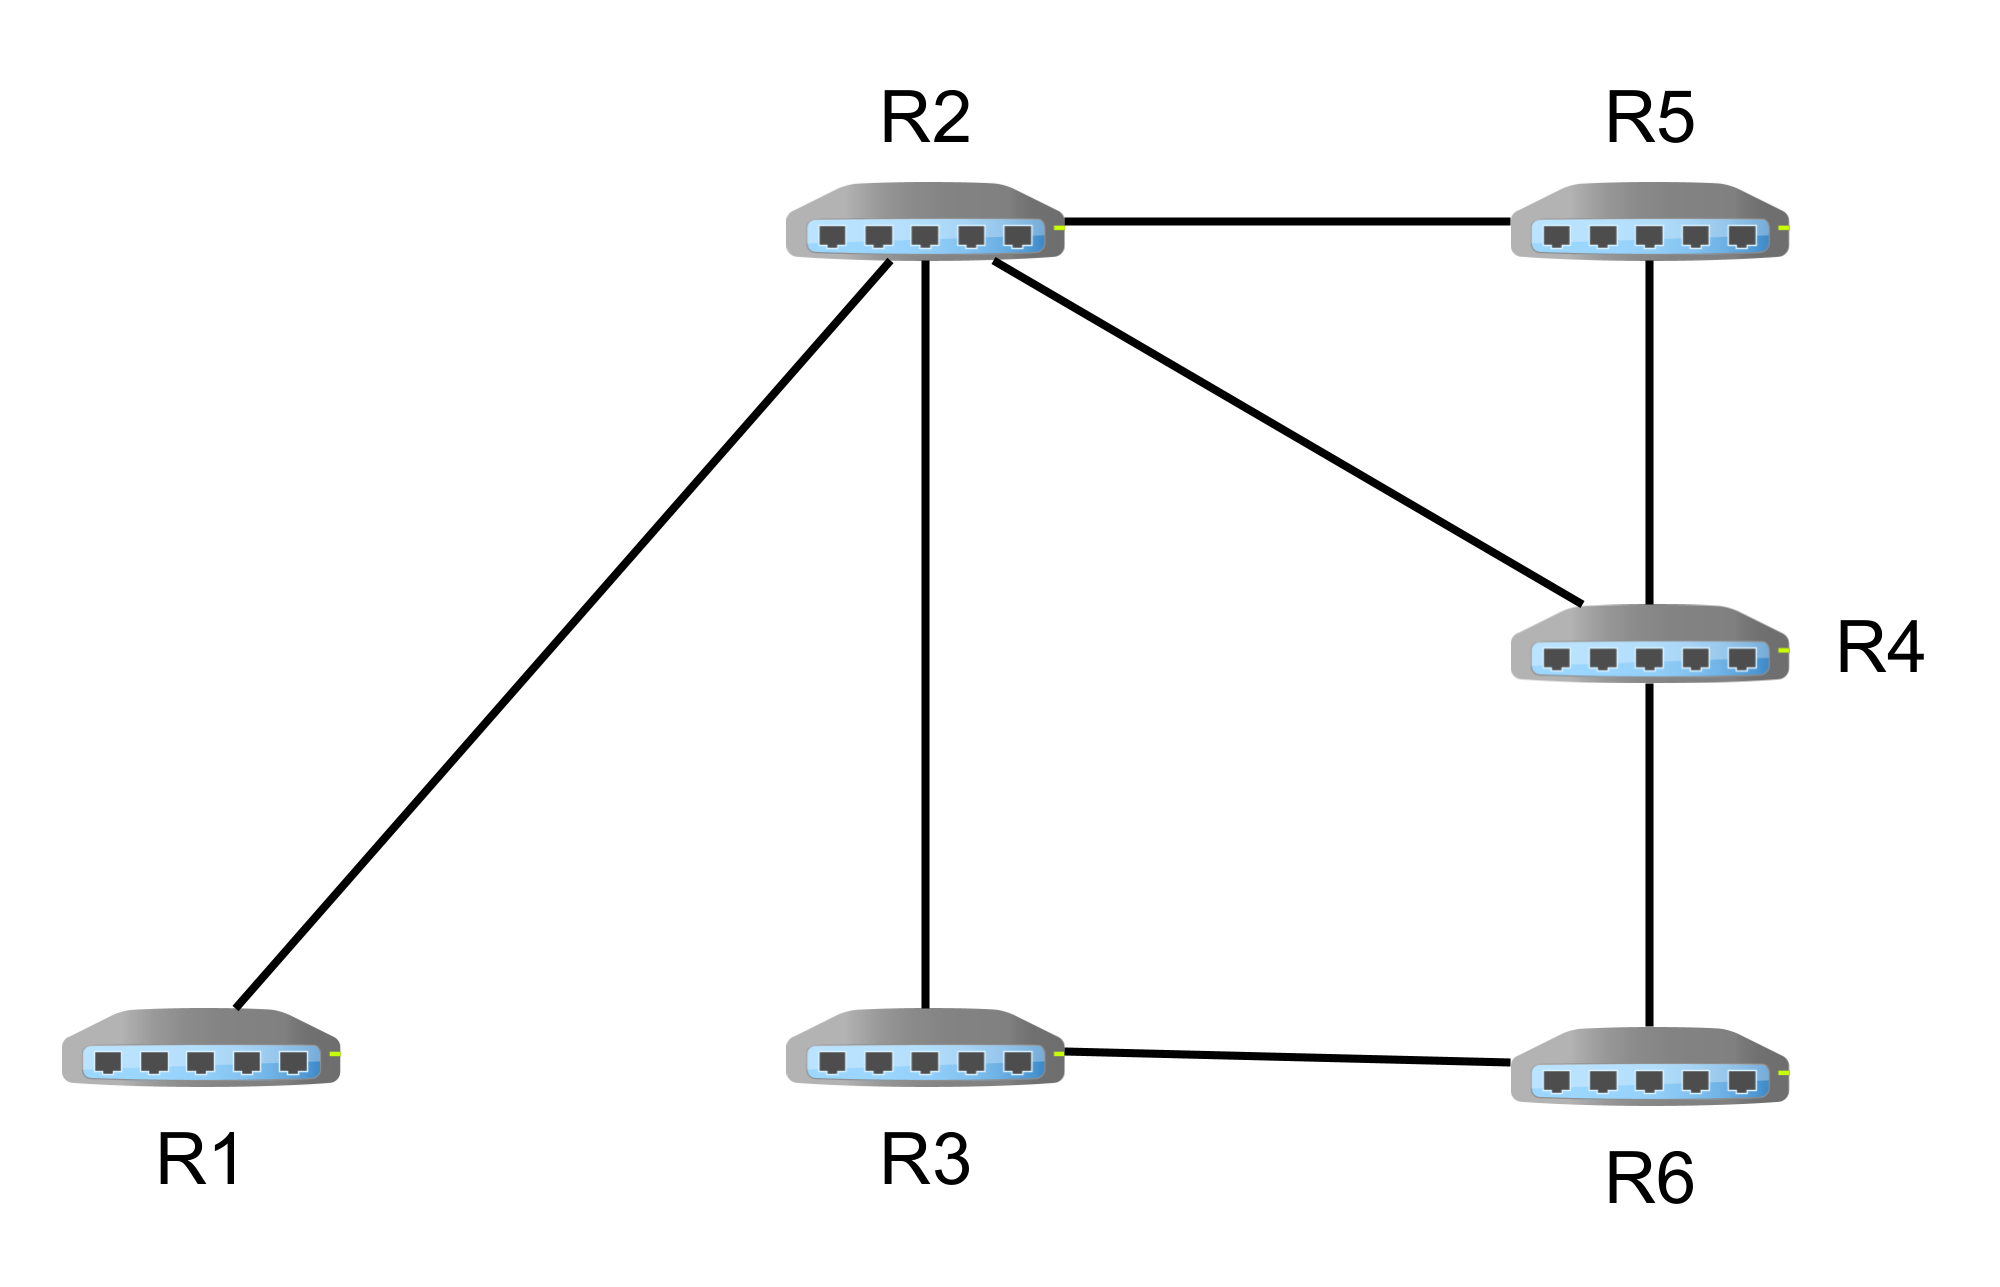
\includegraphics[width=6cm]{img/res1.png}
\end{center}

Donner étape par étape l'évolution des tables de routage de R1 et R6.
\end{exercice}

\begin{exercice}[ : Effet d'une panne]
	On considère le réseau suivant
	\begin{center}
		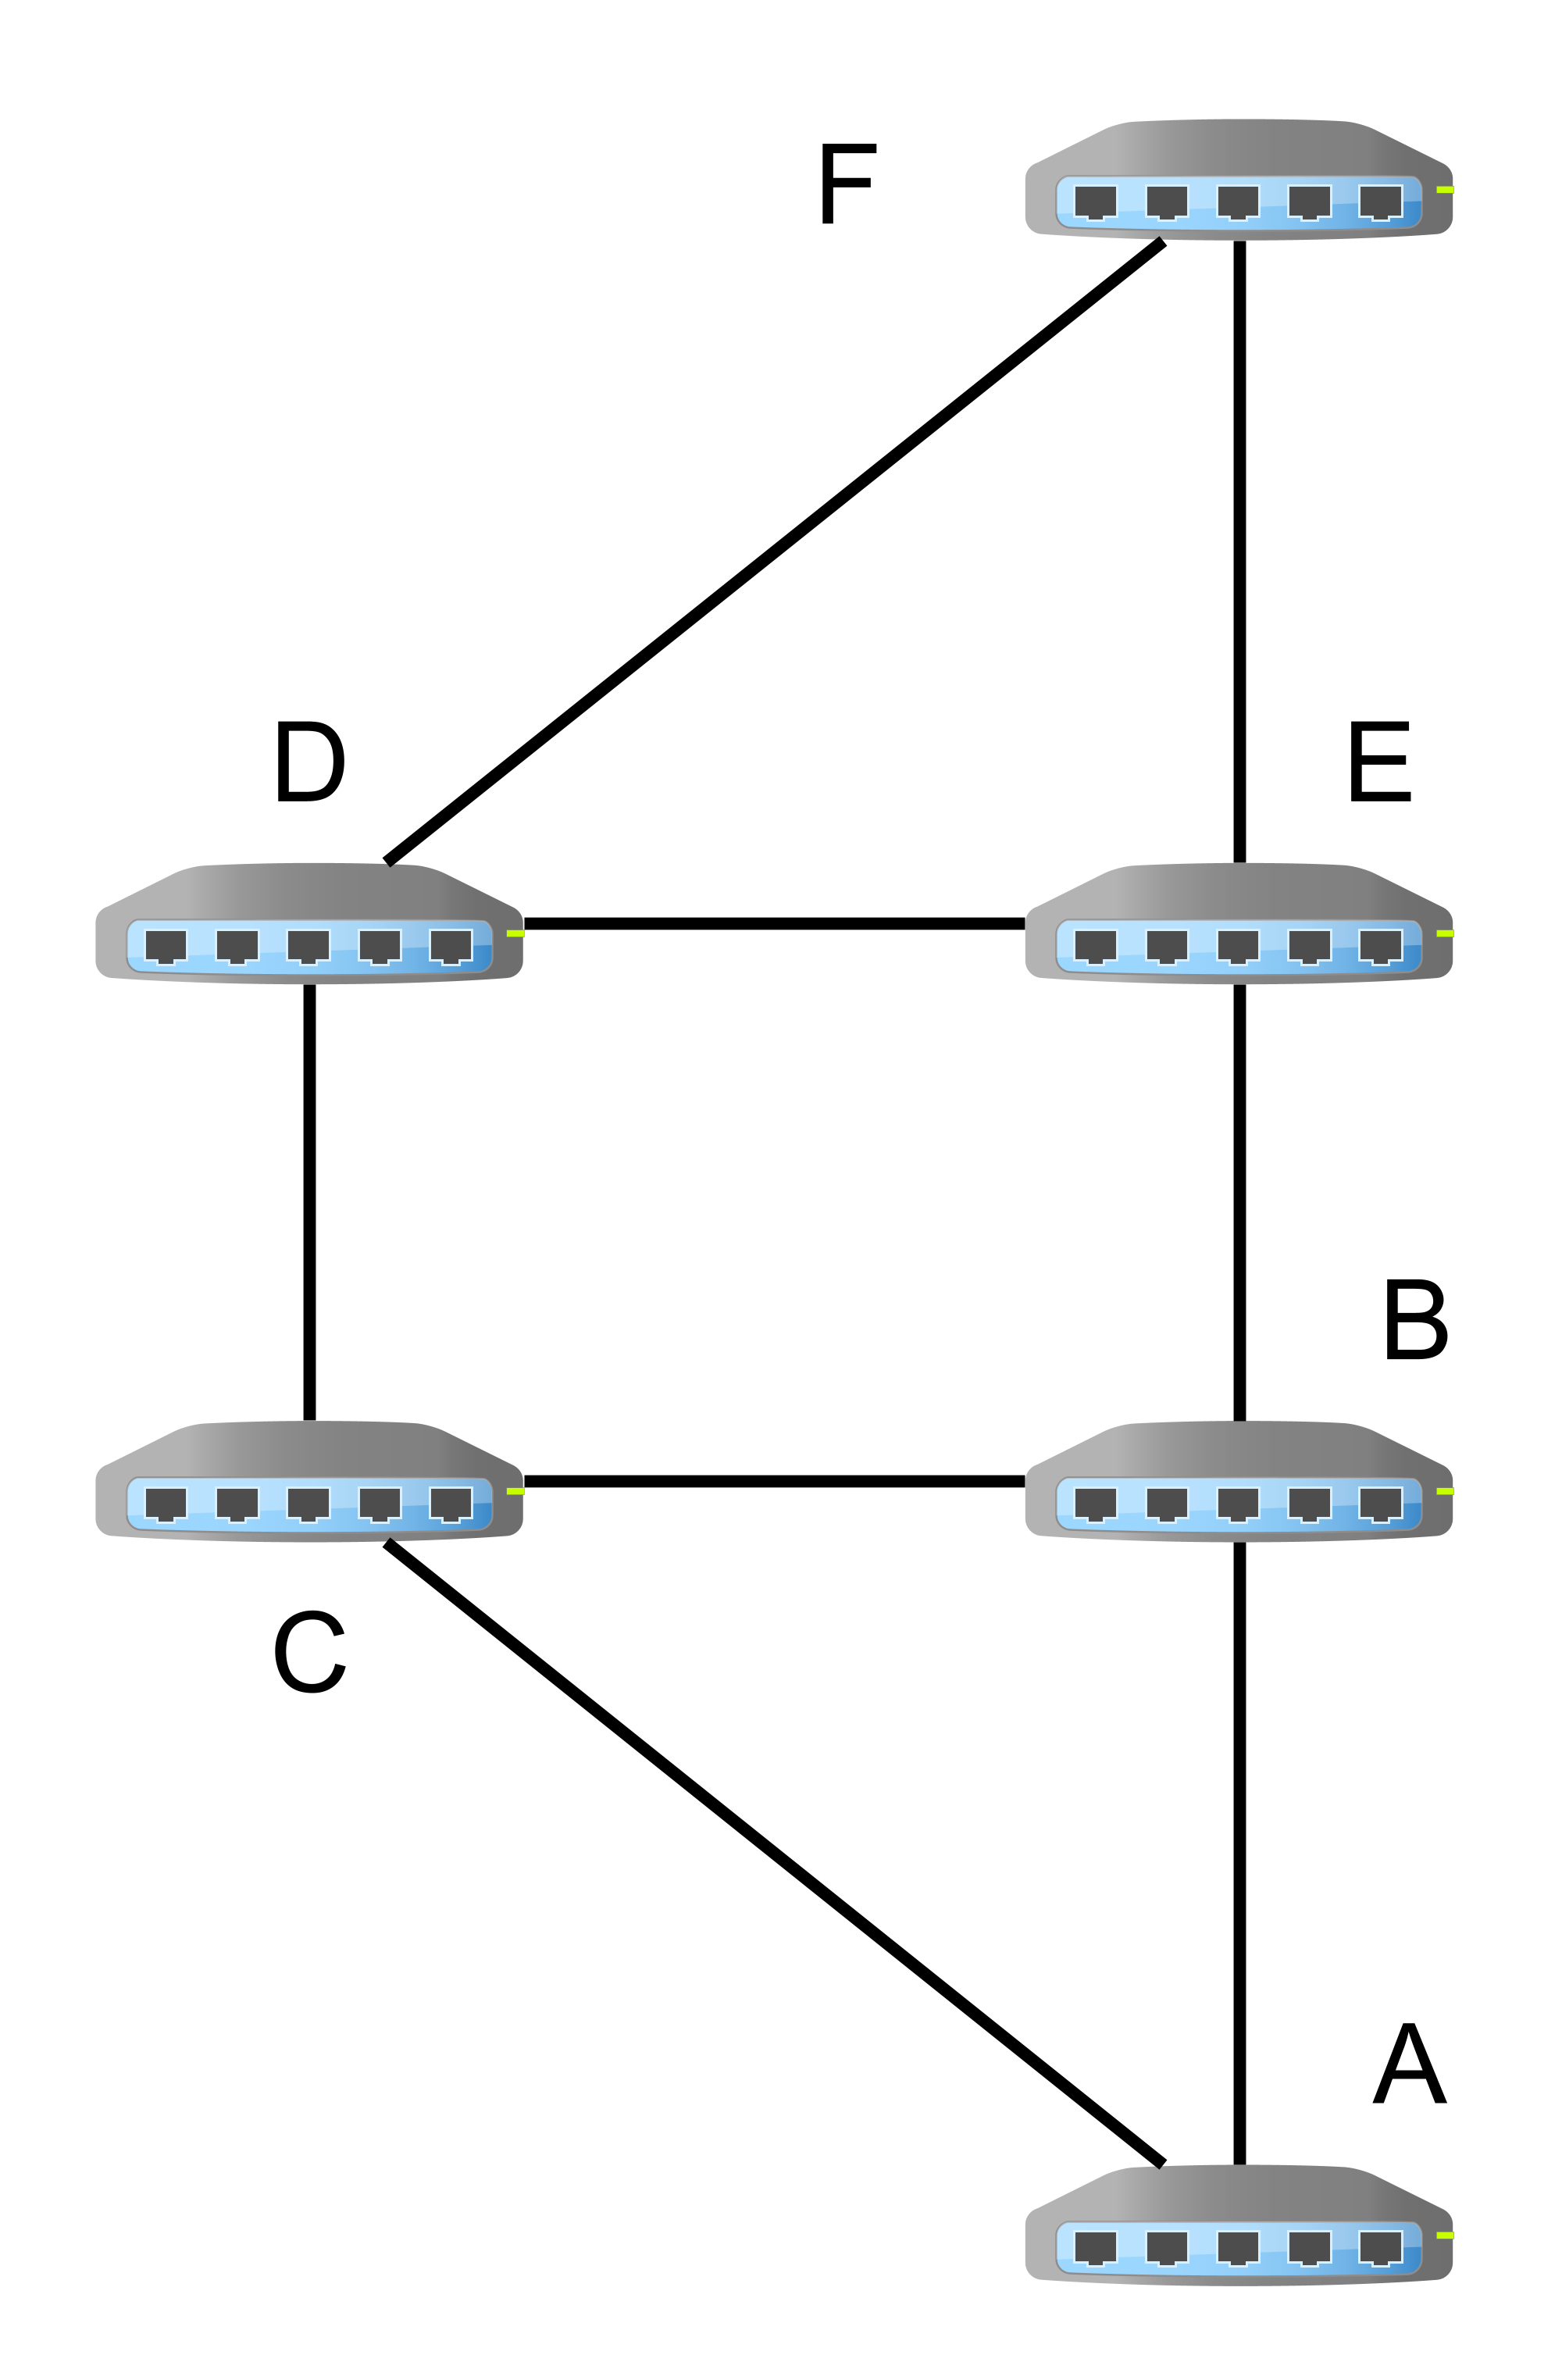
\includegraphics[width=6cm]{img/res2.png}
	\end{center}
	
	Voici la table de routage de A
	
\begin{center}
\begin{tabular}{|c|c|c|}
	\hline
\rowcolor{UGLiOrange}	\textbf{\color{white}Destination} & \textbf{\color{white}Distance} & \textbf{\color{white}Intermédiaire} \\	\hline
	B & 1 & B \\
	\hline
	C & 1 & C \\
	\hline
	D & 2 & C \\	\hline
	E & 2 & B \\	\hline
	F & 3 & B \\
	\hline
\end{tabular}

\end{center}
Le routeur B tombe en panne : il n'emet plus de message RIP.\\
Que va-t-il se passer et comment va évoluer la table de routage de A ?
\end{exercice}

\end{document}